In the last chapter, we have covered means to understand variability,
synthesize variability models for a given software system, and to select sample
sets of configurations. To enable the assessment of performance evolution for
configurable software systems, the next step in our methodology takes into
account the dimension of diachrony. As software evolves, multiple versions, or
called revisions, of a software system exist. In this chapter, we address the
question of how we can assess performance for multiple revisions. Moreover, we
ask whether we can describe a configurable software systems’ performance
evolution without exhaustively assessing all versions by selecting only a
sample set of versions. As illustrated in the methodological road-map in
Figure~\ref{fig:roadmap_2}, we summarize these two questions with the task of
revision sampling.

\begin{figure}[h!]
	\centering
	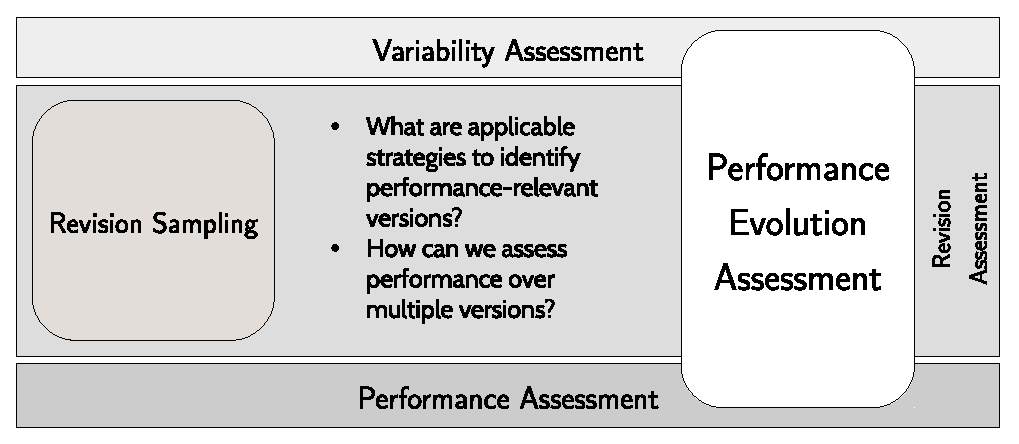
\includegraphics[width=0.75\textwidth]{images/process_revassesment.eps}
	\caption{Methodological road-map: questions to address with revision
	assessment.}
	\label{fig:roadmap_2}
\end{figure}

The chapter is organized as follows. In section~\ref{sec:towards_revsampling} we
present the methodological requirements for a designing and selecting a revision sampling
strategy. In section ~\ref{sec:revsampling_strat} we propose four approaches to
revision sampling based on observations of configurable software systems. In
section~\ref{sec:revsampling_eval} we evaluate the different approaches against
exhaustive measurements of a selection of configurable software systems.
Finally, in section~\ref{sec:revsampling_method} we conclude the chapter and
discuss the approaches' applicability in the context of our methodology.

\section{Towards Revision Sampling}\label{sec:towards_revsampling}
Research so far has addressed the assessment of a software system’s revision
history under the umbrella of repository mining, for instance, to localize bugs
\citep{moin_bug_2010} or performance regression \citep{heger_automated_2013}.
Nonetheless, so far there exists little to no research addressing the question
what the choice of versions might reveal about performance evolution. The task
of selecting resources and a sample set of versions to analyze can be conceived
as a sampling strategy, where the objective is to cover interesting entities
(performance changes, in our case) while trying to limit the sample size to
keep the required effort reasonable. Before we present different approaches to
select a sample set of revisions, we need to define general cornerstones for
evaluating a sample set of revisions as well as respective revision sampling
strategies with respect to performance change history.

\paragraph{Revision Sample Set.} The first question is, what criteria we take as
a basis for rating a sample set of revisions as \emph{meaningful}. First, our intention
is to obtain a representative description of a software system’s performance
change history while only assessing a fraction of revisions. That is, assessing
a representative sample of revisions should yield a performance change history
similar to the assessment of all revisions. Since we are interested in
revisions for which performance measurements change, these revisions should be
contained in a representative sample. Second, especially in the context of
variability, a performance change might only affect a subset of the assessed
configurations. A representative sample set, therefore, should describe a
history of significant performance changes with respect to all variants
assessed. We consider a performance change to be significant, if it affects a
significant portion of the sample of variants (\emph{effect range}) and if the
relative change in performance measurements is significantly large (\emph{effect
magnitude}).

\begin{figure}[h!]
	\centering
	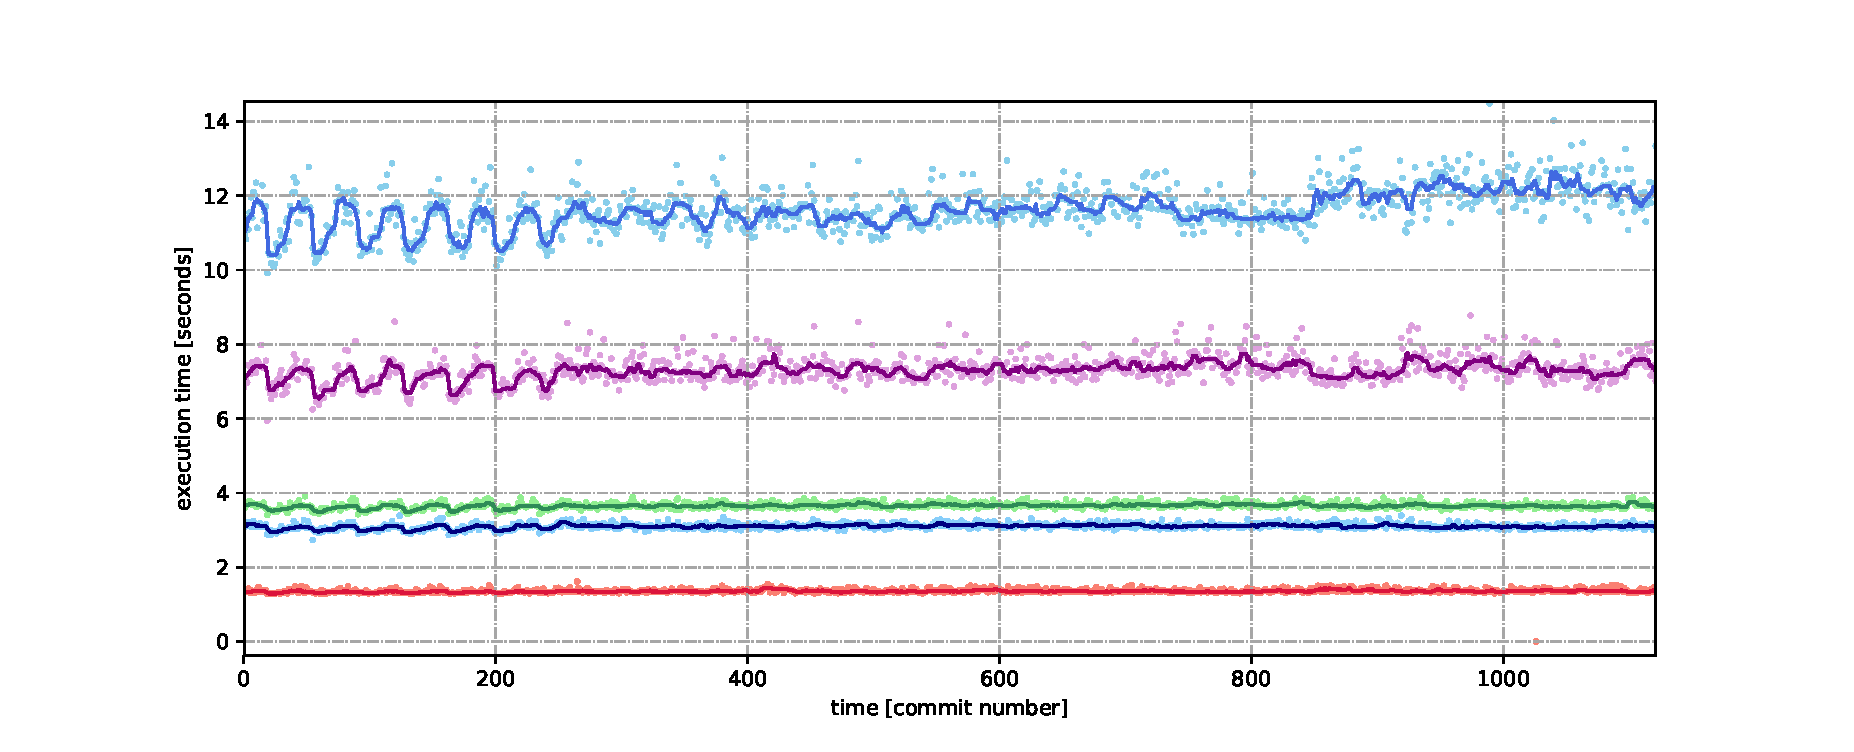
\includegraphics[width=0.95\textwidth]{images/xz_sample_evolution.eps}
	\caption{Performance History for XZ}
	\label{fig:xz_evosample}
\end{figure}

To illustrate the two facets of performance changes, in
Figure~\ref{fig:xz_evosample} we see a history of performance measurements (execution time in this case) for a
small-scale configurable software system, file compression tool called \emph{GNU
XZ Utils}. The graphic depicts execution time measures for executing a standard
compression benchmark for $1,135$ different versions and covers a version
history of about nine years. 

In this excerpt, we only show the execution time measures of five different
variants, i.e., each version was assessed with five different configurations.
Each performance measurement is depicted by a single marker. In addition, we
provide a plot of a moving median, to identify trends. We see that each variant
has a certain performance level, and overall, the performance measurements
remain stable. While the blue and purple variant are generally more volatile,
for all variants, we see performance measurements oscillating during the first
250 versions. With regard to the two facets of significance mentioned earlier,
not all variants are affected similarly by this effect to the same degree.

While the former significance criterion can unambiguously defined by a threshold
number of variants, for the latter one one needs to define how to summarize
relative performance change among all variants. For instance, a performance
change may have a significant magnitude, if the average deviation of
performance measurements for all variants is greater than a specified threshold
value.

\paragraph{Revision Sampling Strategies.} The second question addresses the
rationale behind a revision sampling strategy. To obtain representative sample sets, sampling
strategies are intended to utilize knowledge about the total volume to select
sample sets from. For instance, pair-wise sampling aims to cover most feature
interactions. Similarly, we demand for a meaningful revision sampling strategy
to exhibit a certain rationale or coverage criterion. If we conceive a sampling
strategy as a binary classificator that, in our case, decides whether in a
revision a performance change is likely, or performance measurements might have
changed compared to prior commits, we want  this classifier to be sensitive,
i.e., to have a preferably high true positive rate. That is, a sampling
strategy is meaningful if we learn which revision features most likely indicate
performance changes.\\

In conclusion, when designing a revision sampling strategy, we ask for a
plausible rationale or coverage criterion with respect to performance changes.
A resulting sample set of revisions, in addition, is representative, if the
contained revisions sketch performance changes. For the context of this
methodology, we remain with a clear definition of what performance
changes are significant. Based on these assumptions, in the next section we
propose a selection of four revision sampling approaches based on different
observations.
 
\section{Revision Sampling Strategies}\label{sec:revsampling_strat}

\begin{figure}[t]
\centering
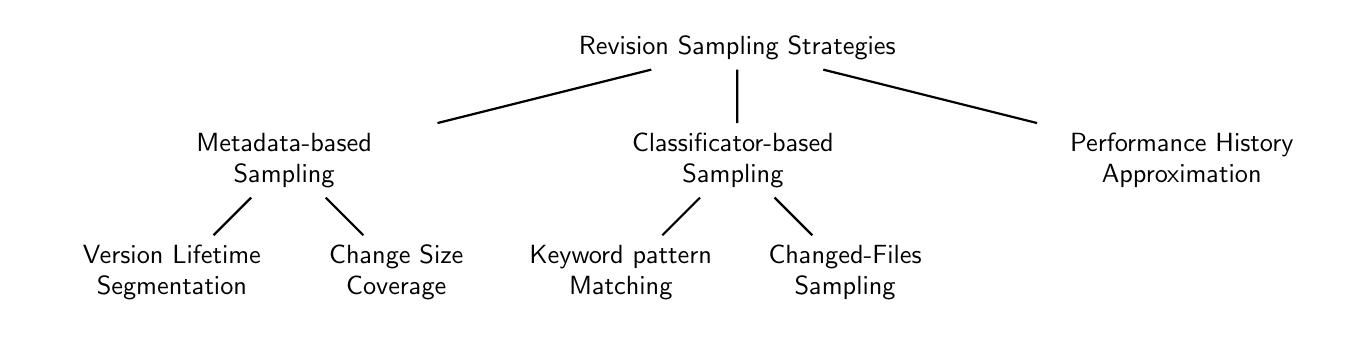
\begin{tikzpicture}[%sibling distance=15em,
level 1/.style={sibling distance=6cm},
level 2/.style={sibling distance=3cm}, 
level 3/.style={sibling distance=6cm},
  every node/.style = {rounded corners,
    draw, align=center,
    top color=white, bottom color=blue!20},thick,scale=0.95, every
    node/.style={scale=0.95}]
  \node {\sffamily Revision Sampling Strategies}
    child { 
    	node [align=left] {
    		\begin{tabular}{c} 
    			{\sffamily \parbox{3.2cm}{\centering Metadata-based Sampling}}
    		\end{tabular}
    	}
    	child { 
    		node [align=left] {
    			\begin{tabular}{c} 
    				{\sffamily \parbox{3.2cm}{\centering Version Lifetime Segmentation}}
    			\end{tabular}
    		}
    	}
    	child { 
    		node [align=left] {
    			\begin{tabular}{c} 
    				{\sffamily \parbox{3.2cm}{\centering Change Size Coverage}}
    			\end{tabular}
    		}
    	} 
    }
    child { 
    	node [align=left] {
    		\begin{tabular}{c} 
    			{\sffamily \parbox{3.2cm}{\centering Classificator-based Sampling}}
    		\end{tabular}
    	}
    	child { 
    		node [align=left] {
    			\begin{tabular}{c} 
    				{\sffamily \parbox{3.2cm}{\centering Keyword pattern Matching}}
    			\end{tabular}
    		}
    	}
    	child { 
    		node [align=left] {
    			\begin{tabular}{c} 
    				{\sffamily \parbox{3.2cm}{\centering Changed-Files Sampling}}
    			\end{tabular}
    		}
    	} 
    }
    child { 
    	node [align=left] {
    		\begin{tabular}{c} 
    			{\sffamily \parbox{3.2cm}{\centering Performance History Approximation}}
    		\end{tabular}
    	} 
    };
%    	child { 
%   		node [align=left] {
%	    		\begin{tabular}{c} 
%	    			{\sffamily \parbox{3cm}{\centering Hot-Spot Sampling}}
%	    		\end{tabular}
%    		}
%    	} 
%    };
\end{tikzpicture}

\caption{Overview of our proposed revision
sampling strategies.}\label{fig:revsampling_overview}
\end{figure}

\subsection{Keyword Pattern Matching}
The first version sampling strategy we present is driven by the conception that
a commit message usually summarizes the changes of a commit in terms of what
has been implemented, modified, removed, or what problems have been fixed.
Commit messages can include keywords or phrases that indicate a performance
context, such as ``\textsf{fixed performance bug \ldots}'', or exhibit
information about the version of the software system, such as ``\textsf{bumped
version number to \ldots'}'.
Based on this information, we propose to use pattern matching to check whether a commit
message contains a keyword that might indicate a performance context, or a new
version, respectively. The sampling algorithm works as follows. Given a set of
keywords, such as ``\textsf{performance, bug, fix, slower, faster, \ldots}'', we
first derive the word stems for each keyword. Second, for each commit message, we split the
message into separate words and derive their corresponding word stems. Third,
we match all sets of resulting word stems (one set per commit message) against
the set of keyword sets and retain those commit messages, for which
sufficiently word stems are contained. As these commit messages contain our
previously defined keywords, we select the corresponding commits as our version
sample set.

This approach is simplistic and its accuracy clearly
depends on the quality of the initial selection of the keyword set. Moreover, more sophisticated ways to
compute similarity between texts, such as the tf-idf-measure and various
similarity metrics \citep{huang_similarity_2008}. However, we only propose this
strategy to evaluate the overall applicability of approaches driven by text
similarity to the problem of version sampling.

\subsection{Version Lifetime Segmentation}
The second approach to select sample versions from the history of versions is
based on assumptions and observations obtained via repository mining. The
following approach is driven by the assumption that performance changes are
more likely to occur when the software system is revised frequently in a short
period of time. Not only is this simply due to a higher number of revisions. We
can also assume that if a software system has not been revised for a long
period of time, changes in terms of performance-relevant fixes were not
necessary, or have been deferred. Although postponing performance-relevant
fixes has become sort of a virtue \citep{molyneaux_art_2014}, for the latter
case the can exist other reasons, including organizational constraints or performance
issues being undetected at that time. That is, we assume that those versions
that have been the latest version for a long time due to the absence of changes
as well as the necessity thereof can sketch a software systems performance
history. We do not assume that long-lasting versions introduce performance
changes, but they enable the segmentation of a software systems version history
in a way that it represents a large portion of the software systems lifetime.

\begin{figure}[!htb]
\def\tabularxcolumn#1{m{#1}}
\begin{tabularx}{\linewidth}{@{}cXX@{}}
\centering
\begin{tabular}{cc}
\subfloat[Activity graph for \texttt{GNU XZ}, generated from 1,135 versions
between December 8, 2007, and August 14, 2017.]
{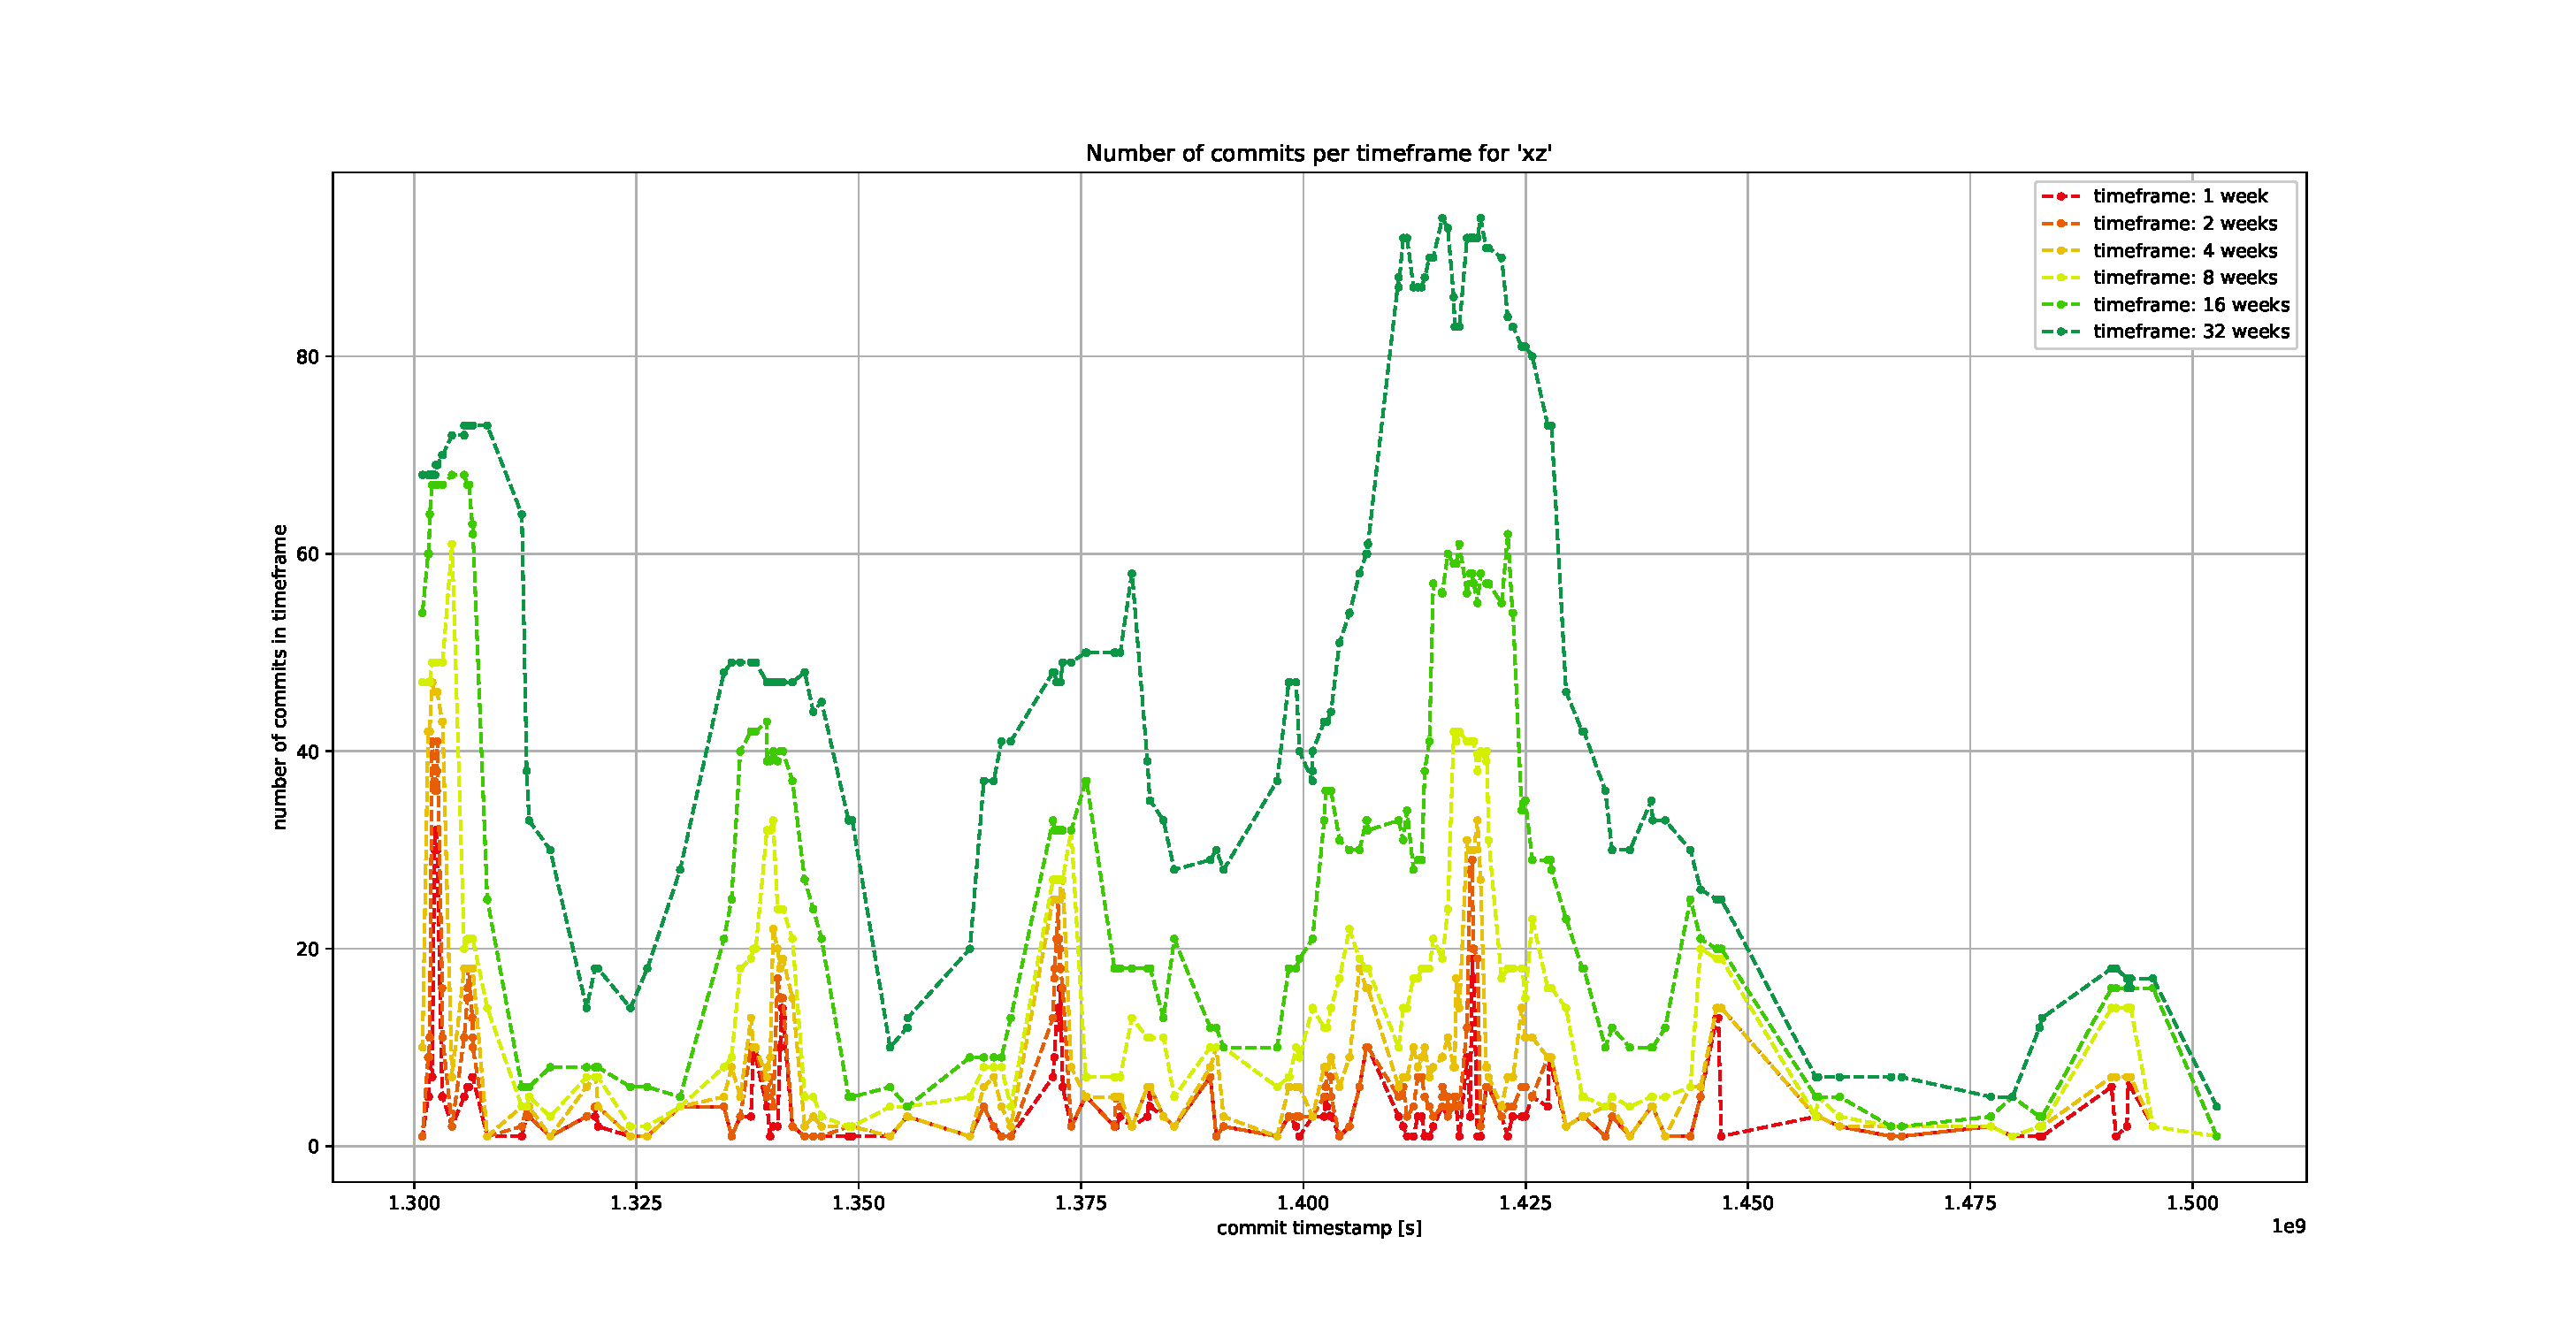
\includegraphics[width=0.45\textwidth]{images/activity_xz.eps}}
&
\subfloat[Activity graph for \texttt{x264}, generated from 2,851 versions
between June 3, 2004, and June 26, 2017.]{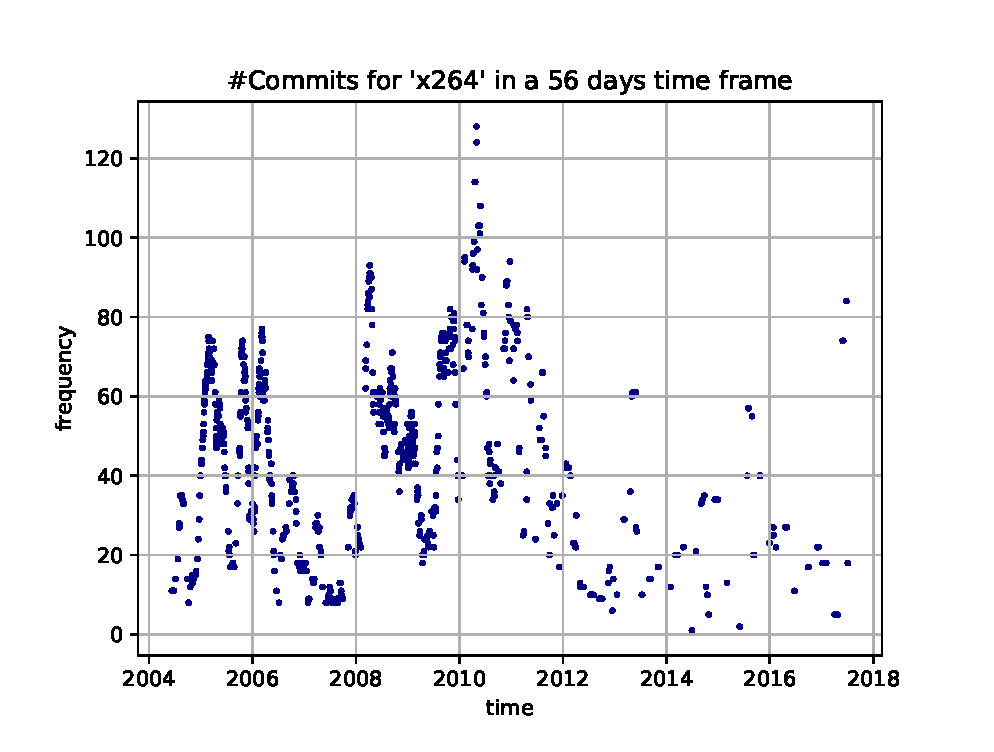
\includegraphics[width=0.45\textwidth]{images/activity_x264.eps}}\\
\end{tabular}
\end{tabularx}
\caption{Commit activity for two sample systems, the compression
utility \texttt{GNU XZ} and the video encoder \texttt{x264}. For each version,
the activity is measured as the number of commits that were pushed within a
certain timeframe of eight weeks.}
\label{fig:ActivityGraphs}
\end{figure}

Making the connection with our methodological context and the aim to design a
version sampling strategy, we intend to achieve a high “lifetime coverage” with
a small number of versions. For this reason, we have evaluated the “lifetime”
of versions of different software systems. In the following, lifetime of a
version or commit refers to the period of time between a commit and its
successor. We have investigated the distribution of version lifetime for two
open-source software systems, a free file compression tool, \emph{GNU XZ}, and a
free video encoder, \emph{x264}. – This selection is by far not representative, yet
the observations obtained from systems document our assumptions. Since we will
refer to those two and other systems for the evaluation, we answer how and why
these systems were selected in the evaluation in chapter 5.  – The first
observation regarding the lifetime of single versions is illustrated in
Figure~\ref{fig:ActivityGraphs} for the two software systems, respectively. The
figure, for each version, shows the activity during development of both systems.
For each commit, we have counted the number of commits preceding and succeeding
it within a four week time frame, respectively. One can see that for both
software systems we can identify spikes with a high commit frequency as well as
plunges with little to no commit activity. Moreover, if we look at the
histogram of all commits lifetime for both systems respectively as illustrated
in Figure~\ref{fig:version_lifetime}, we see that there actually are many
commits with a short lifetime (activity spikes) as well as only very few commits with a long lifetime (plunges).

\begin{figure}[!htb]
\def\tabularxcolumn#1{m{#1}}
\begin{tabularx}{\linewidth}{@{}cXX@{}}
\centering
\begin{tabular}{cc}
\subfloat[Distribution of time to next commits for \texttt{GNU XZ}]
{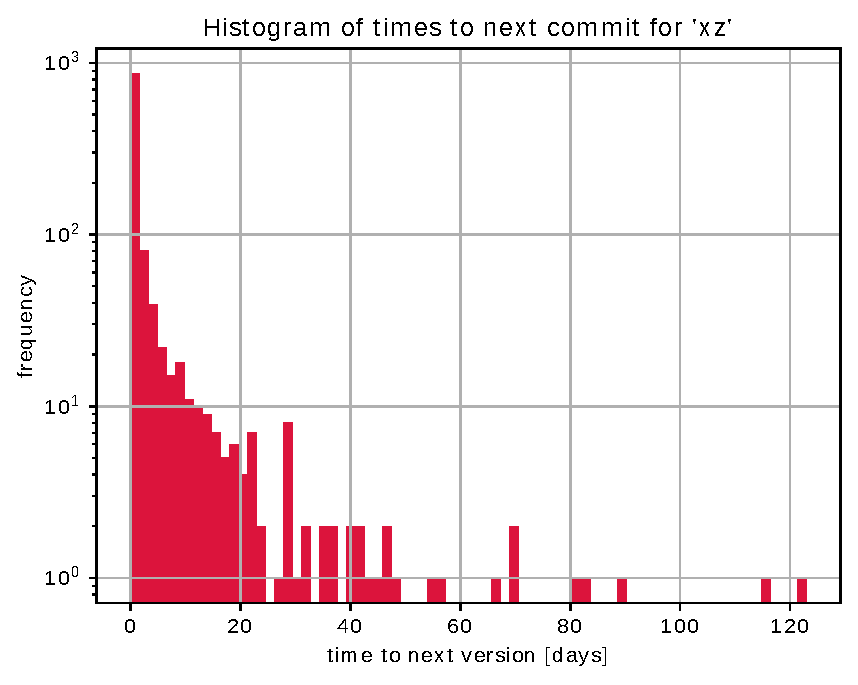
\includegraphics[width=0.45\textwidth]{images/commit_differences_xz.eps}}
&
\subfloat[Distribution of time to next commits for \texttt{x264}]
{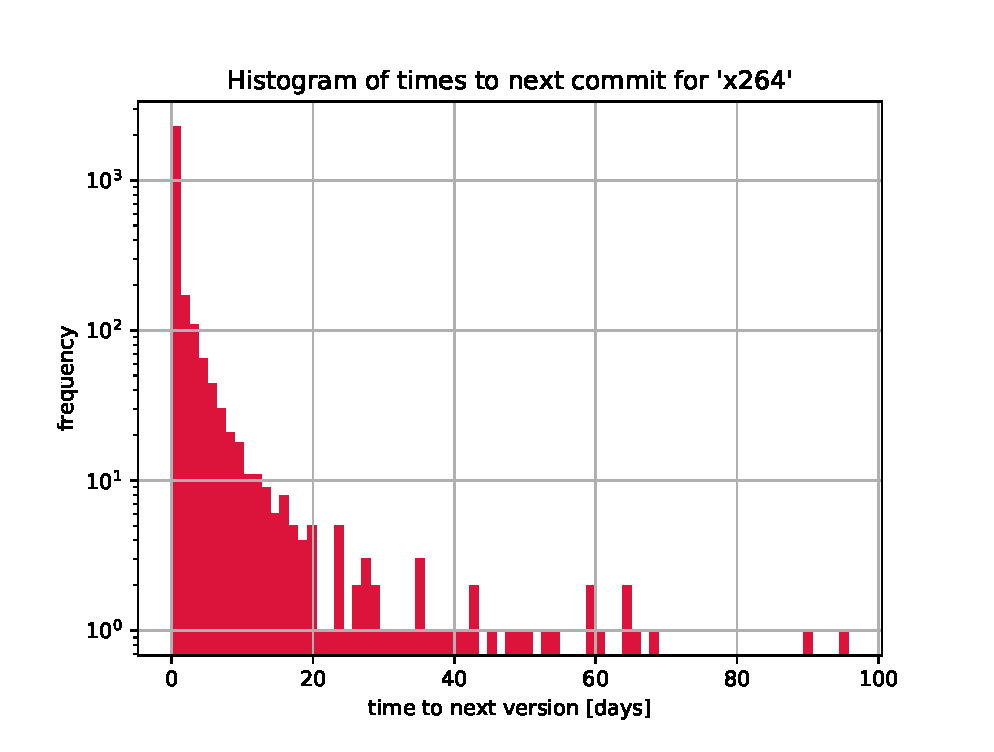
\includegraphics[width=0.45\textwidth]{images/commit_differences_x264.eps}}\\
\end{tabular}
\end{tabularx}
\caption{Distribution of time to next commits for two configurable software
systems, measured as the distance between a commit and its successor.}
\label{fig:version_lifetime}
\end{figure}

Based on the aforementioned assumptions as well as the distribution of version
lifetimes, when translating this in the context of a version sampling strategy,
we can achieve high ``lifetime coverage''  by selecting very few versions from a
list of versions sorted by lifetime in descending order. This sampling strategy
picks the longest-lasting commits until a desired coverage threshold, or
version threshold number is reached. This sample selection of commits is a
segmentation or clustering of the overall version history. We assume that each
segment represents a (sort of) steady state of the software systems performance
history.

\subsection{Change Size Coverage}
The third approach we propose adapts the idea of the previously mentioned
version lifetime segmentation. The following sampling strategy design is driven
by the assumption that a version or commit is more likely to introduce
performance changes to a software system if it modifies a large portion of
code. We assume that the effect of modifying a single line of code is not as
significant as modifying multiple lines of code. Of course, modifications can
accumulate, or trigger already existing interactions, yet from a black-box
perspective, commits affecting more lines of code are more likely to introduce
performance changes or to trigger interactions. That is, for designing a
version sampling strategy, we aim to cover most of all changes made to the
software system with a few number of versions. Similar to the assessment of
version lifetime in Figures~\ref{fig:ActivityGraphs} and
\ref{fig:version_lifetime}, we have investigated the distribution of commit
sizes in terms of lines of code for the two software systems \emph{GNU XZ} and
\emph{x264}. As illustrated in Figure~\ref{fig:version_size}, we see that, by far, most
commits modify less than 2,000 lines of code, whereas very few commits modify
or add larger code sections.

\begin{figure}[!htb]
\def\tabularxcolumn#1{m{#1}}
\begin{tabularx}{\linewidth}{@{}cXX@{}}
\centering
\begin{tabular}{cc}
\subfloat[Distribution of changed lines per commit for \texttt{GNU XZ}]
{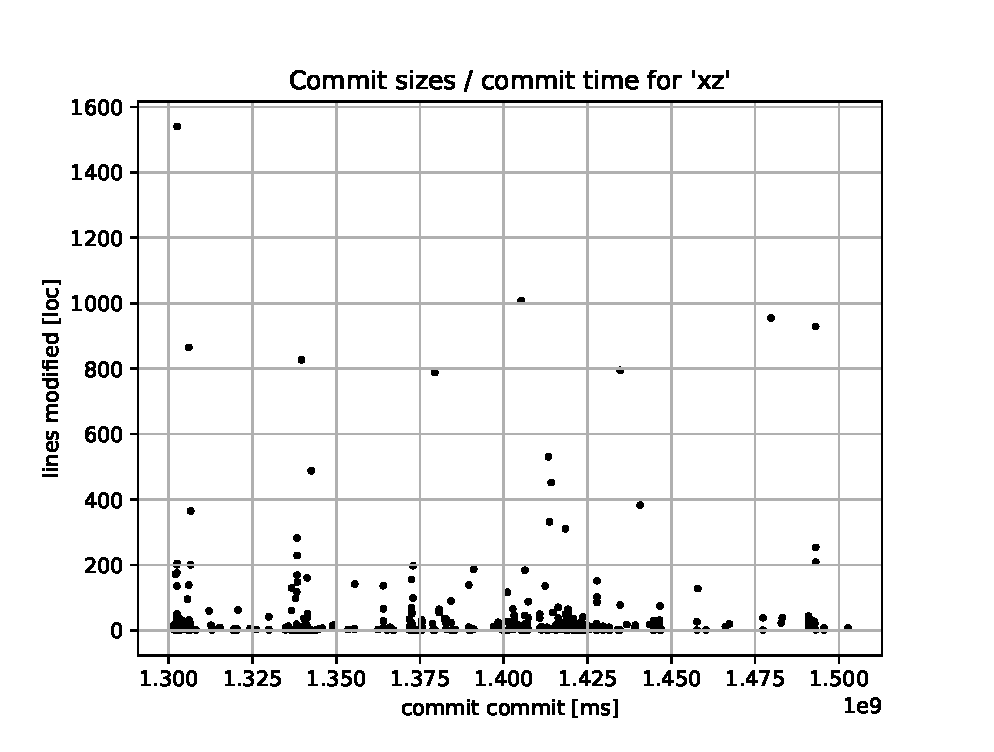
\includegraphics[width=0.45\textwidth]{images/commit_sizes_xz.eps}}
&
\subfloat[Distribution of changed lines per commit for \texttt{x264}]{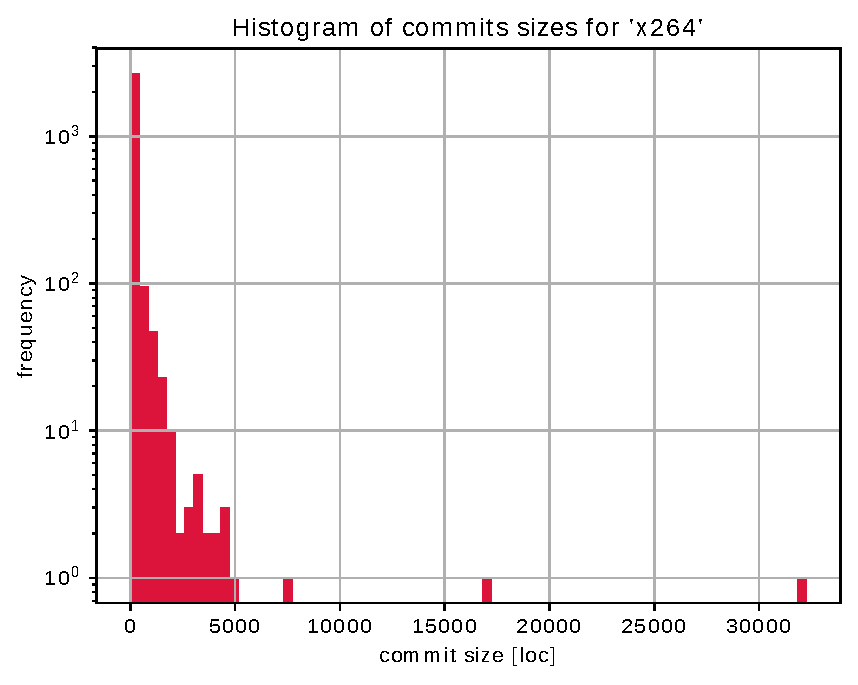
\includegraphics[width=0.45\textwidth]{images/commit_sizes_x264.eps}}\\
\end{tabular}
\end{tabularx}
\caption{Distribution of commit sizes in lines of code for two configurable
software systems, \texttt{GNU XZ} and \texttt{x264}.}
\label{fig:version_size}
\end{figure}

Based on these observations and given the assumption that larger commits are
more likely to introduce performance changes, we propose to obtain a sample of
versions by selecting versions from a list of versions sorted by commit size in
a descending order. Similarly to version lifetime segmentation, one can specify
a threshold of sample set size or commit size coverage to achieve. We assume
that a sample set of versions obtained using this approach is likely to cover
significant performance changes since a larger portion of the overall change
history is covered.


\subsection{Performance History Approximation}
The next sampling strategy that we propose is an adaption of the revision
sampling approach used by \cite{heger_automated_2013}. For a software system’s version
history along with test cases and corresponding performance measurements, the
authors aim to identify those commits which may have introduced performance
regression. The authors have used a binary-search-like approach to iteratively
bisect the version history to find commits for which performance measurements
deviate significantly from previously measured ones. Once a relevant commit is
identified, it can be subject of further root-cause analysis.

\begin{wrapfigure}{r}{0.5\textwidth}
  \begin{center}
    \vspace{-1cm}
    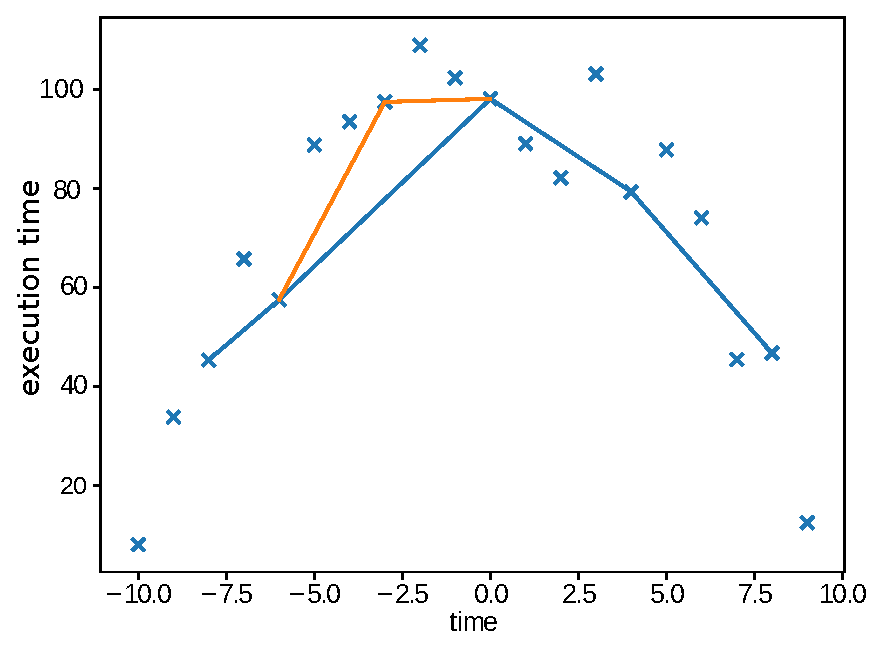
\includegraphics[width=0.48\textwidth]{images/inverse_douglas_peucker}
  \end{center}
  \caption{Given a initial sample of five versions and four segments (blue
  line), the steepest segment is bisected and replaced by two segments (orange).
  The first of the orange segments is steeper than the segment that was
  bisected. \label{fig:example_bisection}}
\end{wrapfigure}

We adapt this approach to extract performance-relevant commits given an initial
sample of versions along with performance measurements. A performance-relevant
commit in this context is a commit for which performance measurements
significantly deviate from measurements of previous commits. The sampling
strategy is applied as follows. Given an initial sample of $n$ versions and
corresponding performance measurements, the version history is segmented into
$n-1$ segments. Each segment is clearly specified by two commits. For each
segment $s_i$, the algorithm now computed the difference in performance measures
$\delta_i$ for the start and the end commit. For the largest differences, the
segment is bisected. For the resulting two segments $\delta_{i_1}$ and
$\delta_{i_2}$, the performance measurement differences are calculated. If the
absolute difference between $\delta_{i_1}$ and  $\delta_{i_2}$ is greater than
zero, one of the two children segments is ``steeper'', i.e. has a greater
performance measurement difference than the parent segment as exemplified in
Figure~\ref{fig:example_bisection}.
One can specify a minimum threshold difference to retain those resulting segments. This procedure
is repeated until no further segments can be bisected without violating the
minimum performance difference threshold. That is, the algorithm approximates
an interpolation of the overall performance history while focusing on sketching
the steepest changes.

\subsection{Changed-Files Sampling}
The last version sampling strategy that we are going to present is a binary
classifier that predicts whether a commit is likely to introduce performance
changes. The idea behind this classifier is that performance changes might
depend on changes in specific code sections or combinations thereof. For each
commit we can retrieve which code sections, or files have been touched. If
there exists a relation between a commit’s file change set and performance
changes, one could learn it and predict performance change likelihood for
arbitrary commits.

We propose a sampling strategy that based on a random initial sample learns a
possible relation between a commit’s set of changed files and performance
changes. For each commit in the initial learning sample, the performance
difference to the previous commit is calculated. Since we are interested in any
change in performance, not only performance degradation, we consider the
absolute performance difference as the performance change introduced by that
commit. Consequently, using classification and regression trees (CARTs), we
approximate a function that maps a commit’s set of changed files to it’s
absolute performance change. If the classificator is accurate enough, it can be
used to select the commits that are most likely to introduce performance
changes.


\section{Strategy Evaluation}\label{sec:revsampling_eval}
\section{Methodological Remarks}\label{sec:revsampling_method}

%\begin{figure}
%\def\tabularxcolumn#1{m{#1}}
%\begin{tabularx}{\linewidth}{@{}cXX@{}}
%\begin{tabular}{c}
%\subfloat[Activity Graph for \texttt{GNU XZ}, generated from 399 versions
%between March 24, 2017, and August 14, 2017. The earliest release version is
%\texttt{5.1.1alpha}, the latest is \texttt{5.3.0alpha}.]
%{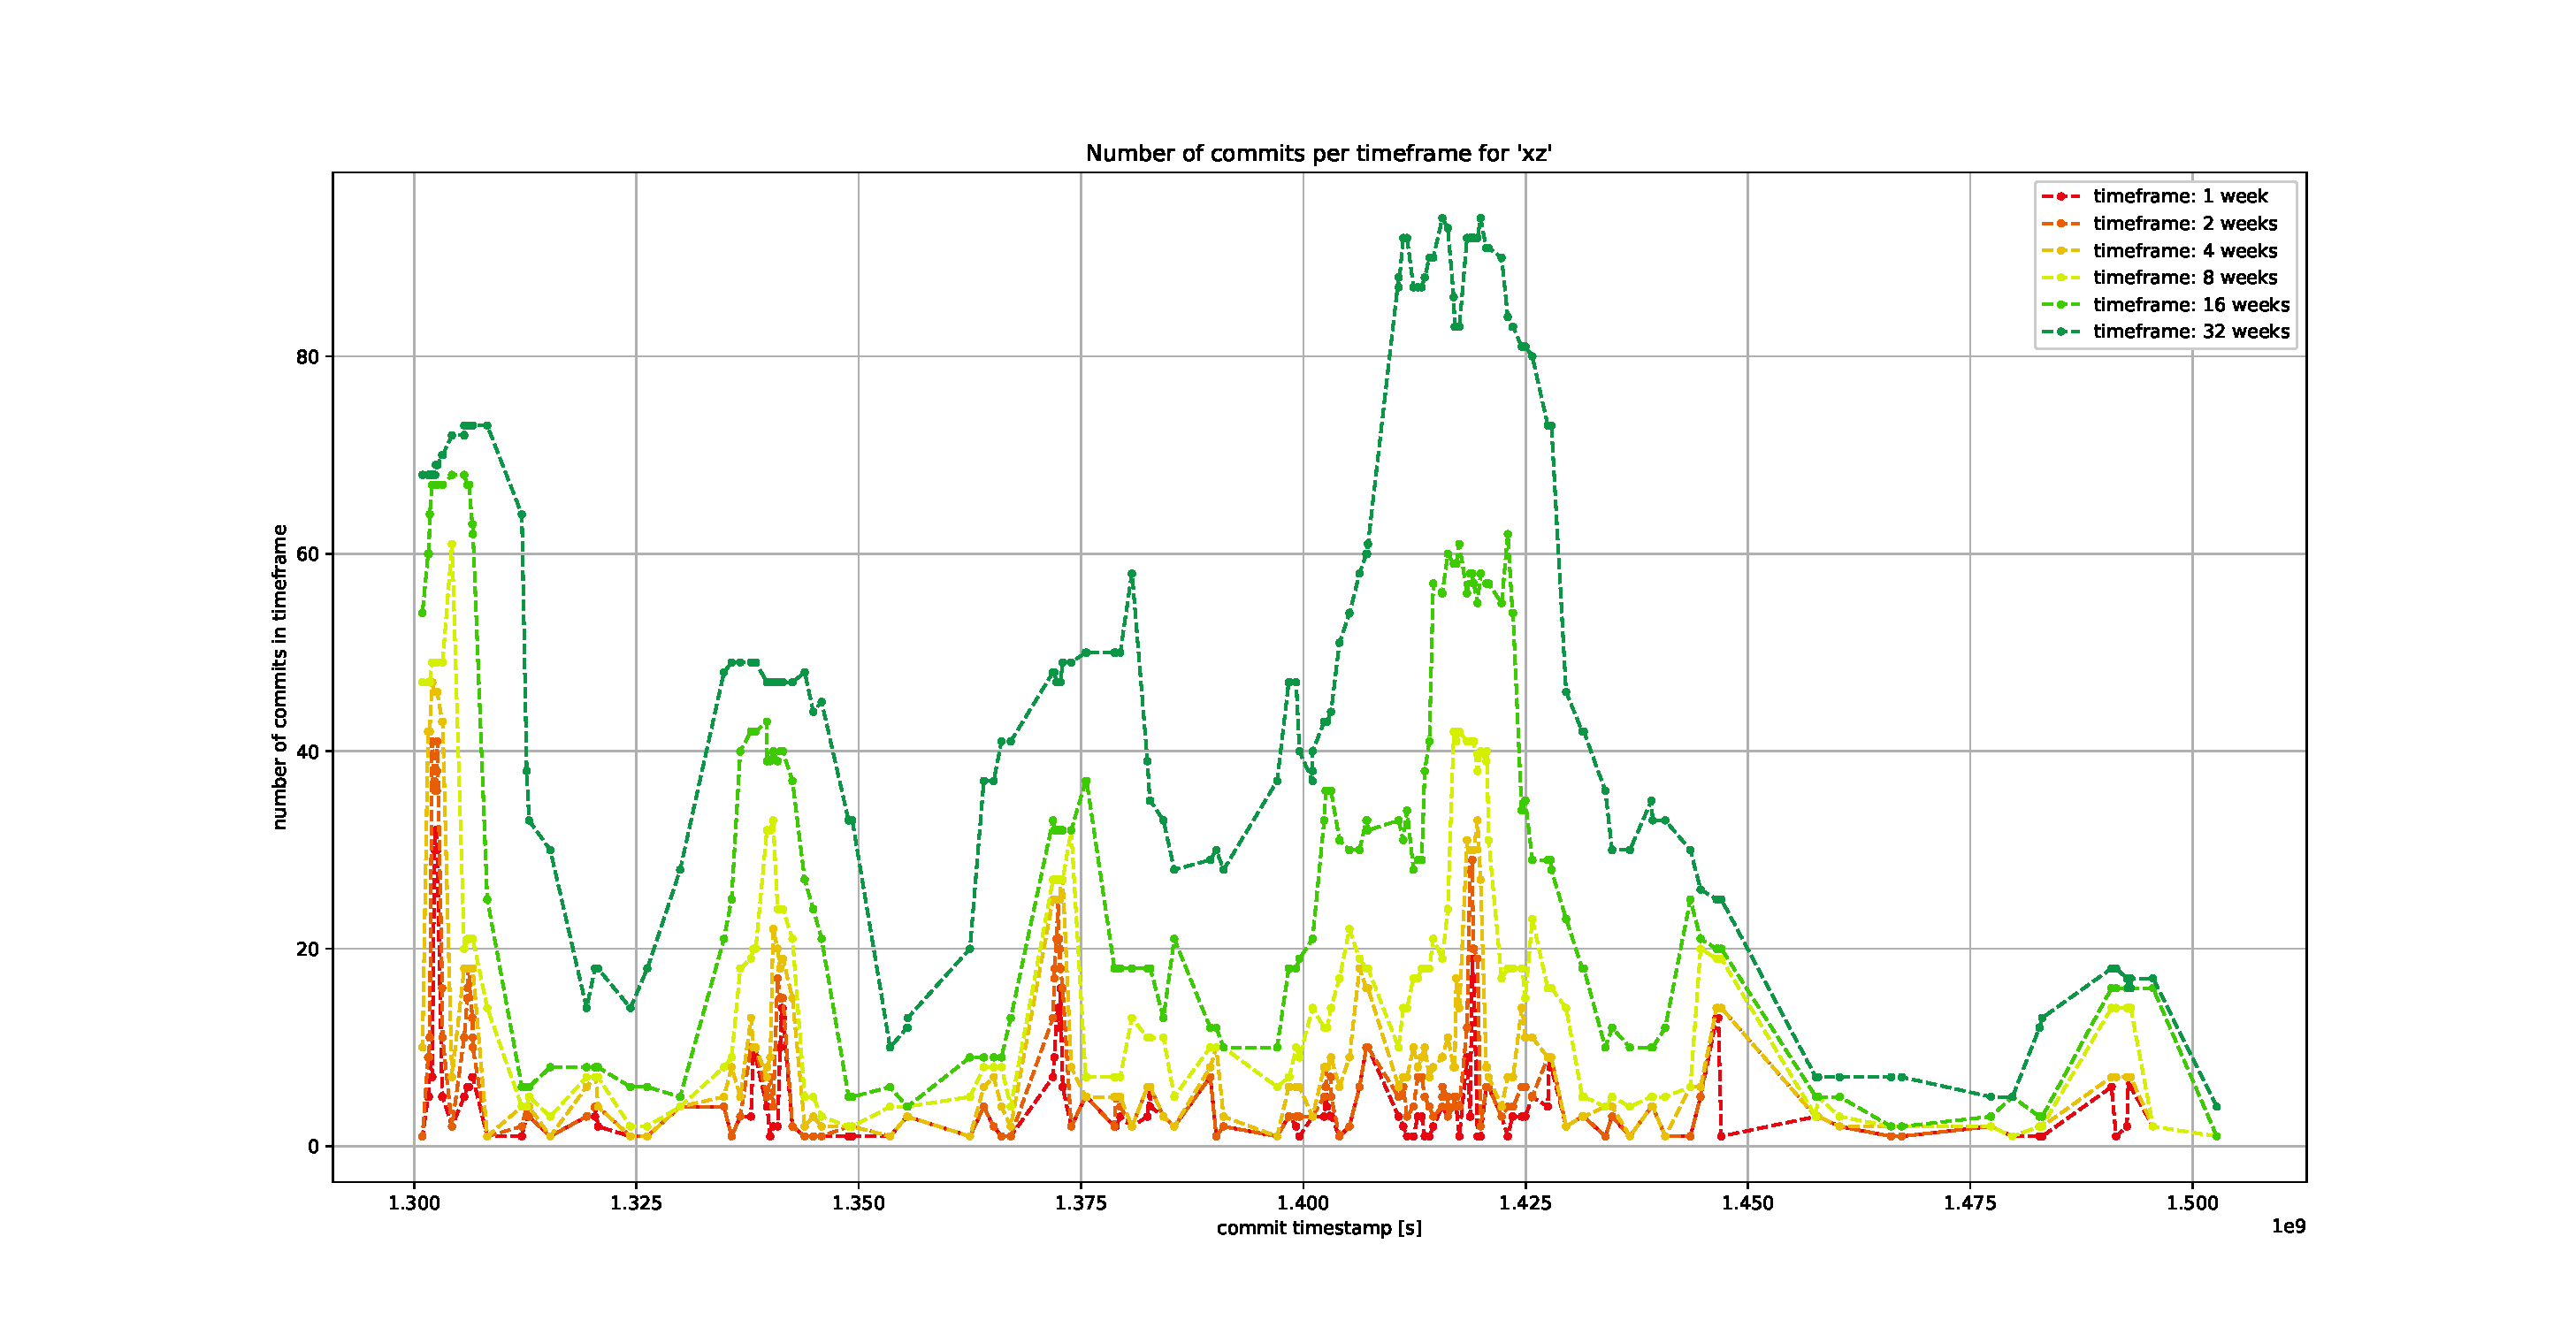
\includegraphics[width=0.99\textwidth]{images/activity_xz.eps}}
%\\
%\subfloat[Activity Graph for \texttt{x264}, generated from 2851 versions
%between June 3, 2004, and June 26, 2017. The earliest release version is
%\texttt{BUILD 1} from, the latest is \texttt{BUILD 149} from
%X.]{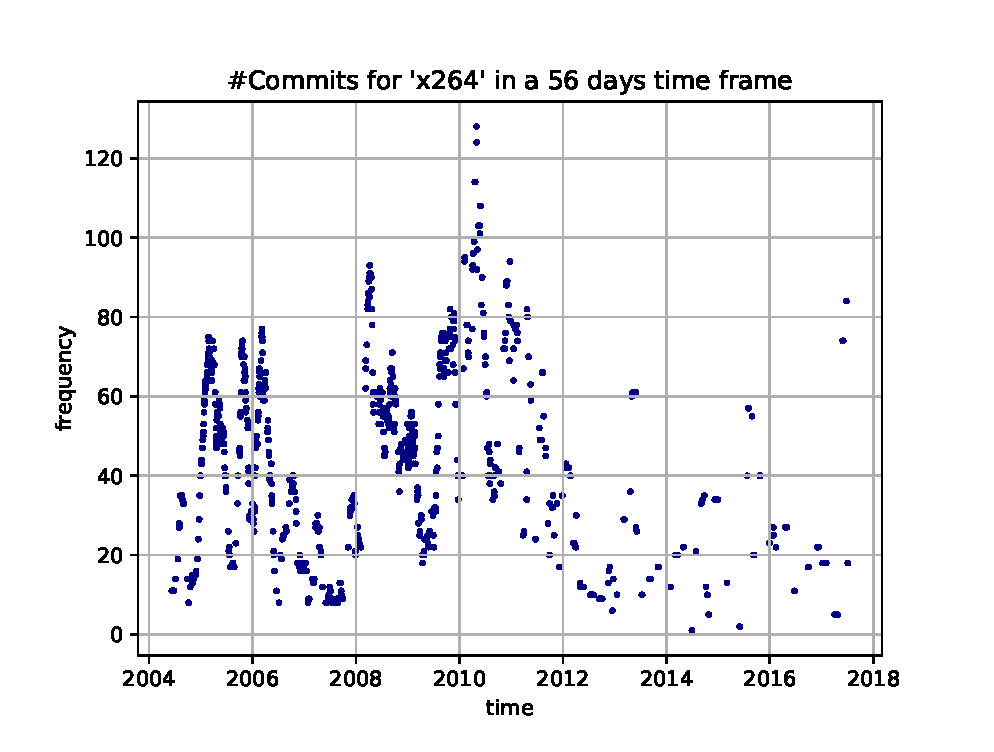
\includegraphics[width=0.99\textwidth]{images/activity_x264.eps}}\\
%\end{tabular}
%\end{tabularx}
%\caption{Commit activity for two sample systems, the compression
%utility \texttt{GNU XZ} and the video encoder \texttt{x264}. For each version,
%the activity is measured as the number of commits that were pushed within a
%certain timeframe after or before the actual commit. The timeframes range from
%one week to 32 weeks, as shown in the legendary.}
%\label{fig:ActivityGraphs}
%\end{figure}
